\newpage
\section{Полученные результаты}
\subsection{Серийные расчёты на структурированной расчётной сетке}
На основе изложенных выше численных методов был реализован программный комплекс для моделирования волновых задач механики деформируемого твёрдого тела. С помощью программного комплекса проведены расчёты различных постановок неразрушающего контроля изотропных и анизотропных композиционных материалов. За образец для расчёта взята обшивка элемента крыла самолёта, изображённая на рис. \ref{pic:construction}. Последовательность углов поворота анизотропных слоёв $45^{\circ}, 0^{\circ}, -45^{\circ}, 0^{\circ}, 0^{\circ}, 90^{\circ}, 0^{\circ}, 0^{\circ}, -45^{\circ}, 0^{\circ}, 45^{\circ}$.

На рис. \ref{pic:general-view} показан общий вид волновой картины в образце с одиннадцатью скрещенными анизотропными слоями с расслоением между вторым и третьим снизу слоями. Ультразвуковой детектор (схематически показан конусом) обновременно является источником и приёмником волн -- попеременный режим работы.
\begin{figure}[H]
	\center{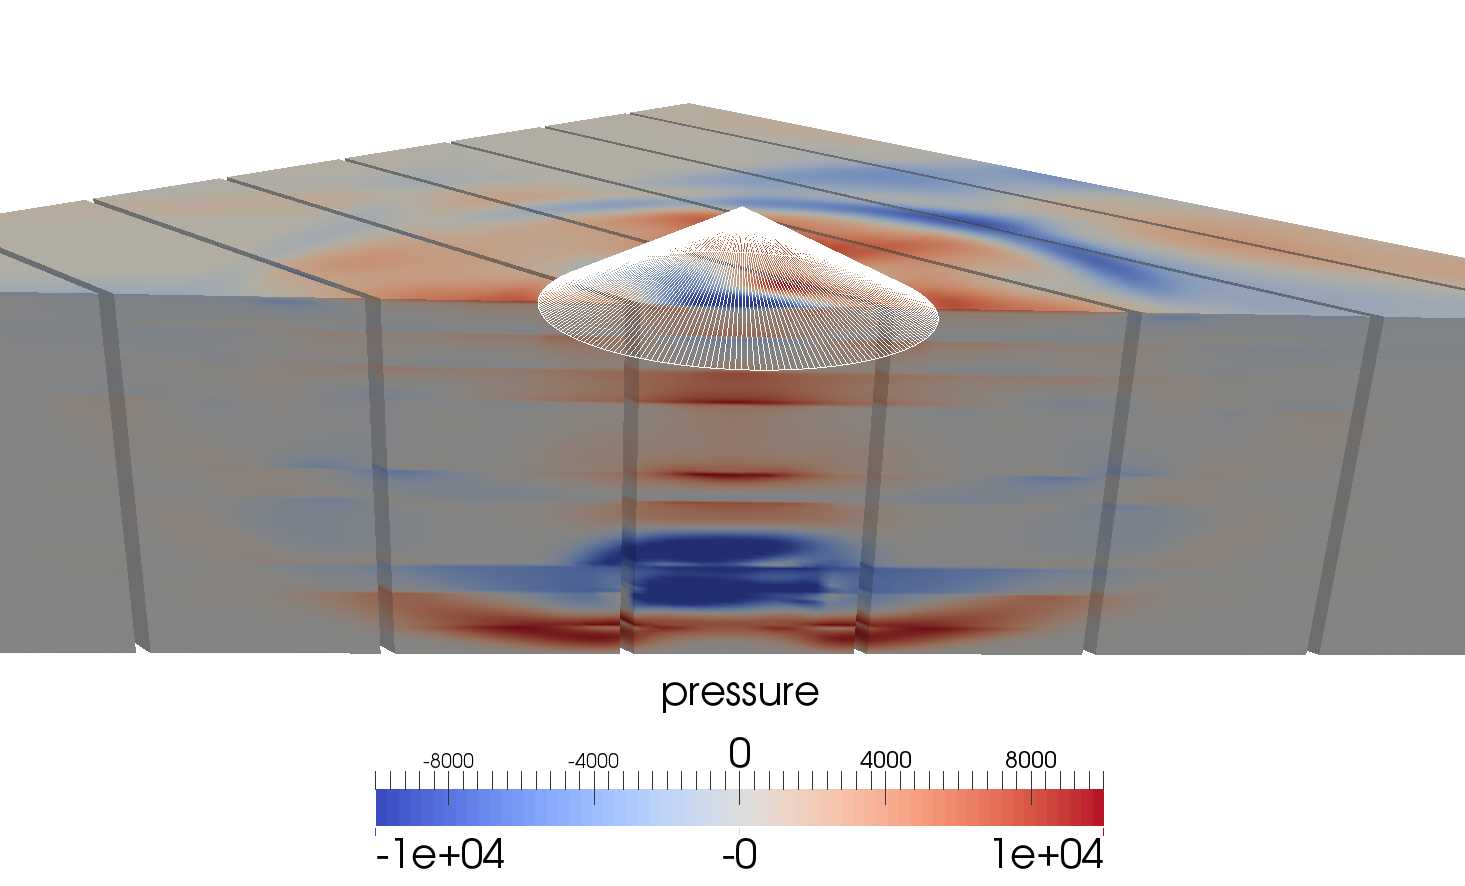
\includegraphics[width=1\textwidth]{png/res/general-view.png}}
	\caption{Общий вид волновой картины при расчёте постановки. Сверху схематически изображён ультразвуковой детектор}
	\label{pic:general-view}
\end{figure}

На рис. \ref{pic:p-wave} показан профиль продольной волны вдоль вертикальной оси при неразрушающем контроле образца с расслоением между вторым и третьим снизу слоями. На рис. \ref{pic:s-wave} -- профиль сдвиговой волны в материале без расслоения.
\begin{figure}%[H]
	\center{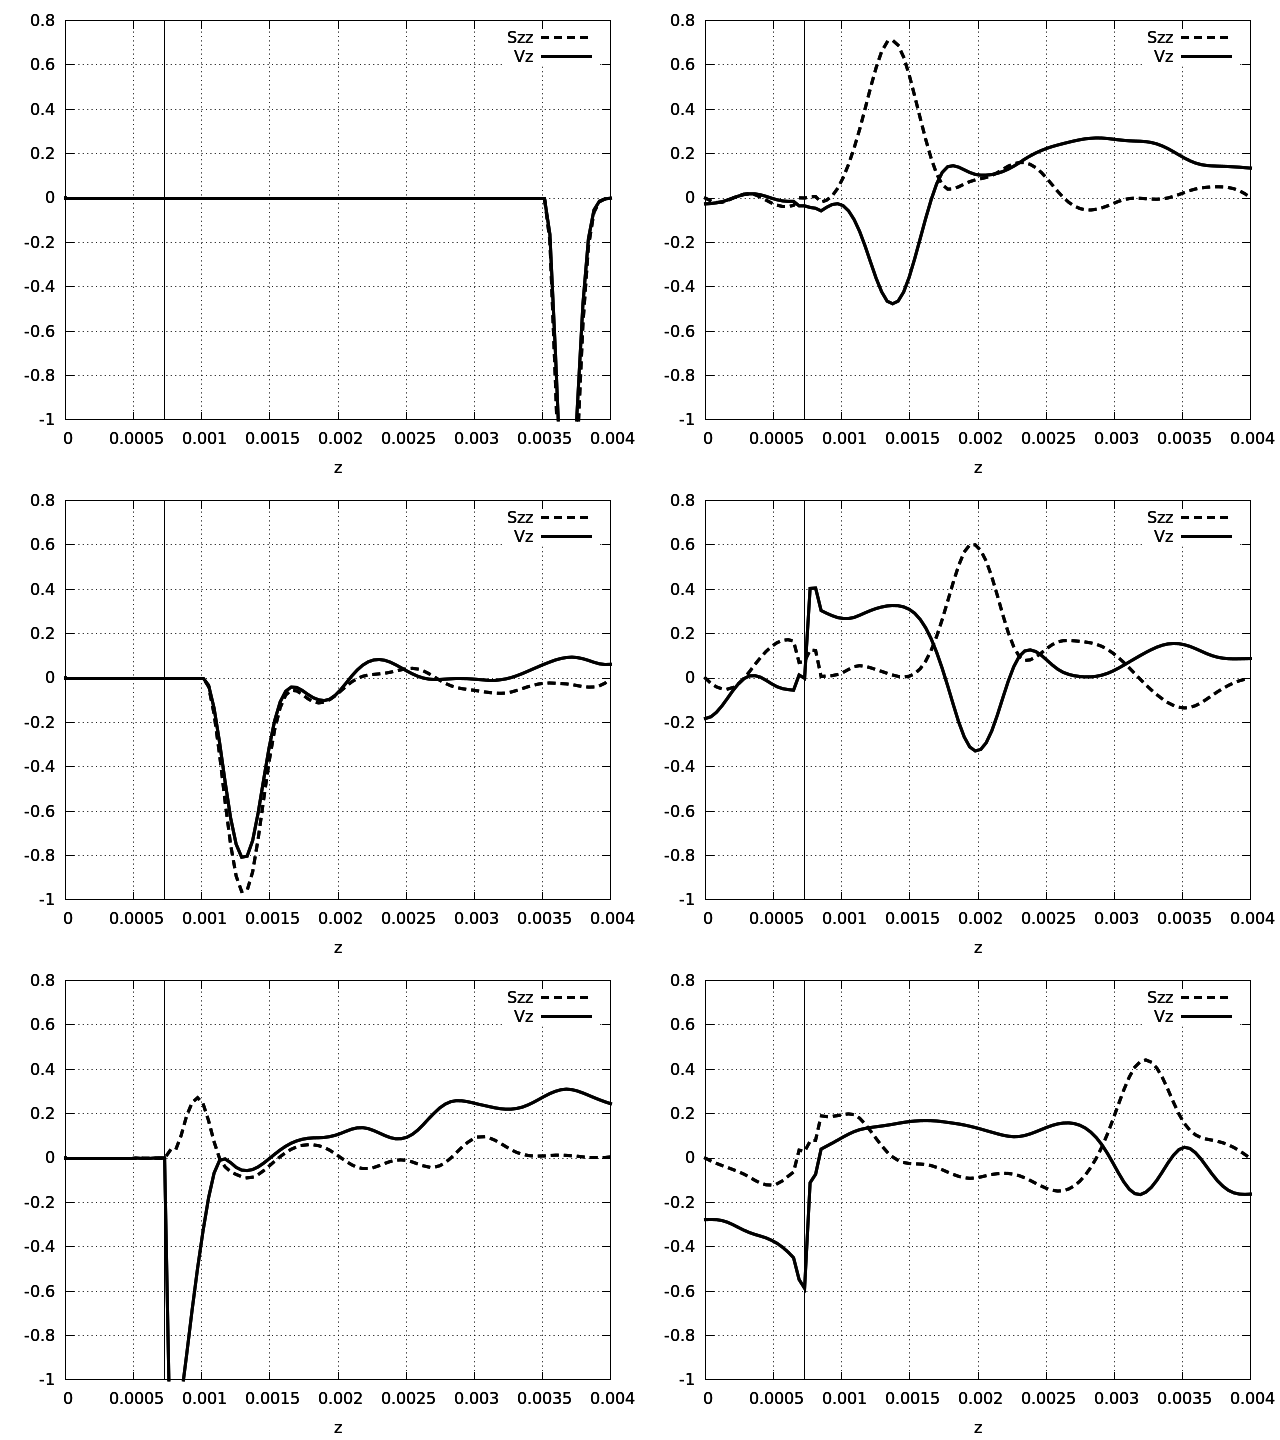
\includegraphics[width=1\textwidth]{png/res/p-wave.png}}
	\caption{Распространение продольной волны вдоль оси $z$ в материале с расслоением. Расслоение показано вертикальной линией. Последовательные моменты времени сверху вниз, слева направо}
	\label{pic:p-wave}
\end{figure}


\begin{figure}%[H]
	\center{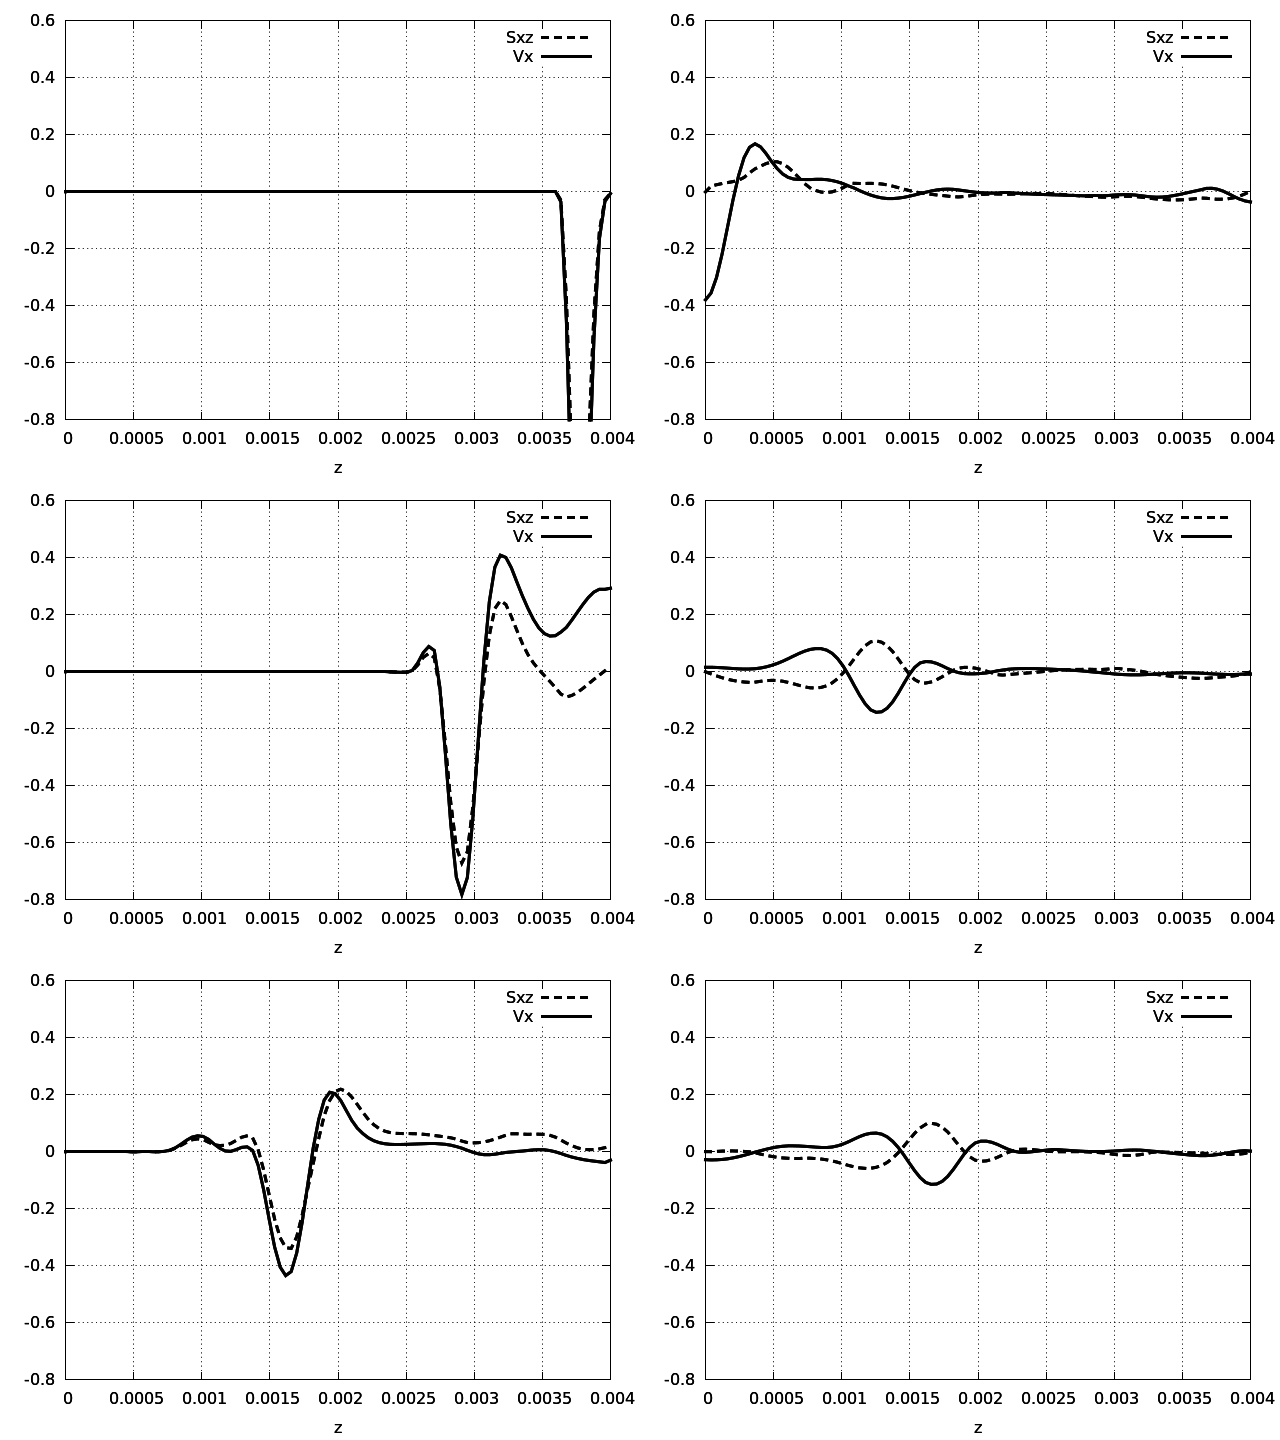
\includegraphics[width=1\textwidth]{png/res/s-wave.png}}
	\caption{Распространение сдвиговой волны вдоль оси $z$ в материале без дефекта. Последовательные моменты времени сверху вниз, слева направо}
	\label{pic:s-wave}
\end{figure}

На рис. \ref{pic:fracture-detection} показаны рассчитанные показания ультразвукового детектора на продольных волнах для образцов с трещинами между разными слоями. По расстоянию между пиками можно определить, между какими слоями произошло расслоение.
\begin{figure}%[H]
	\center{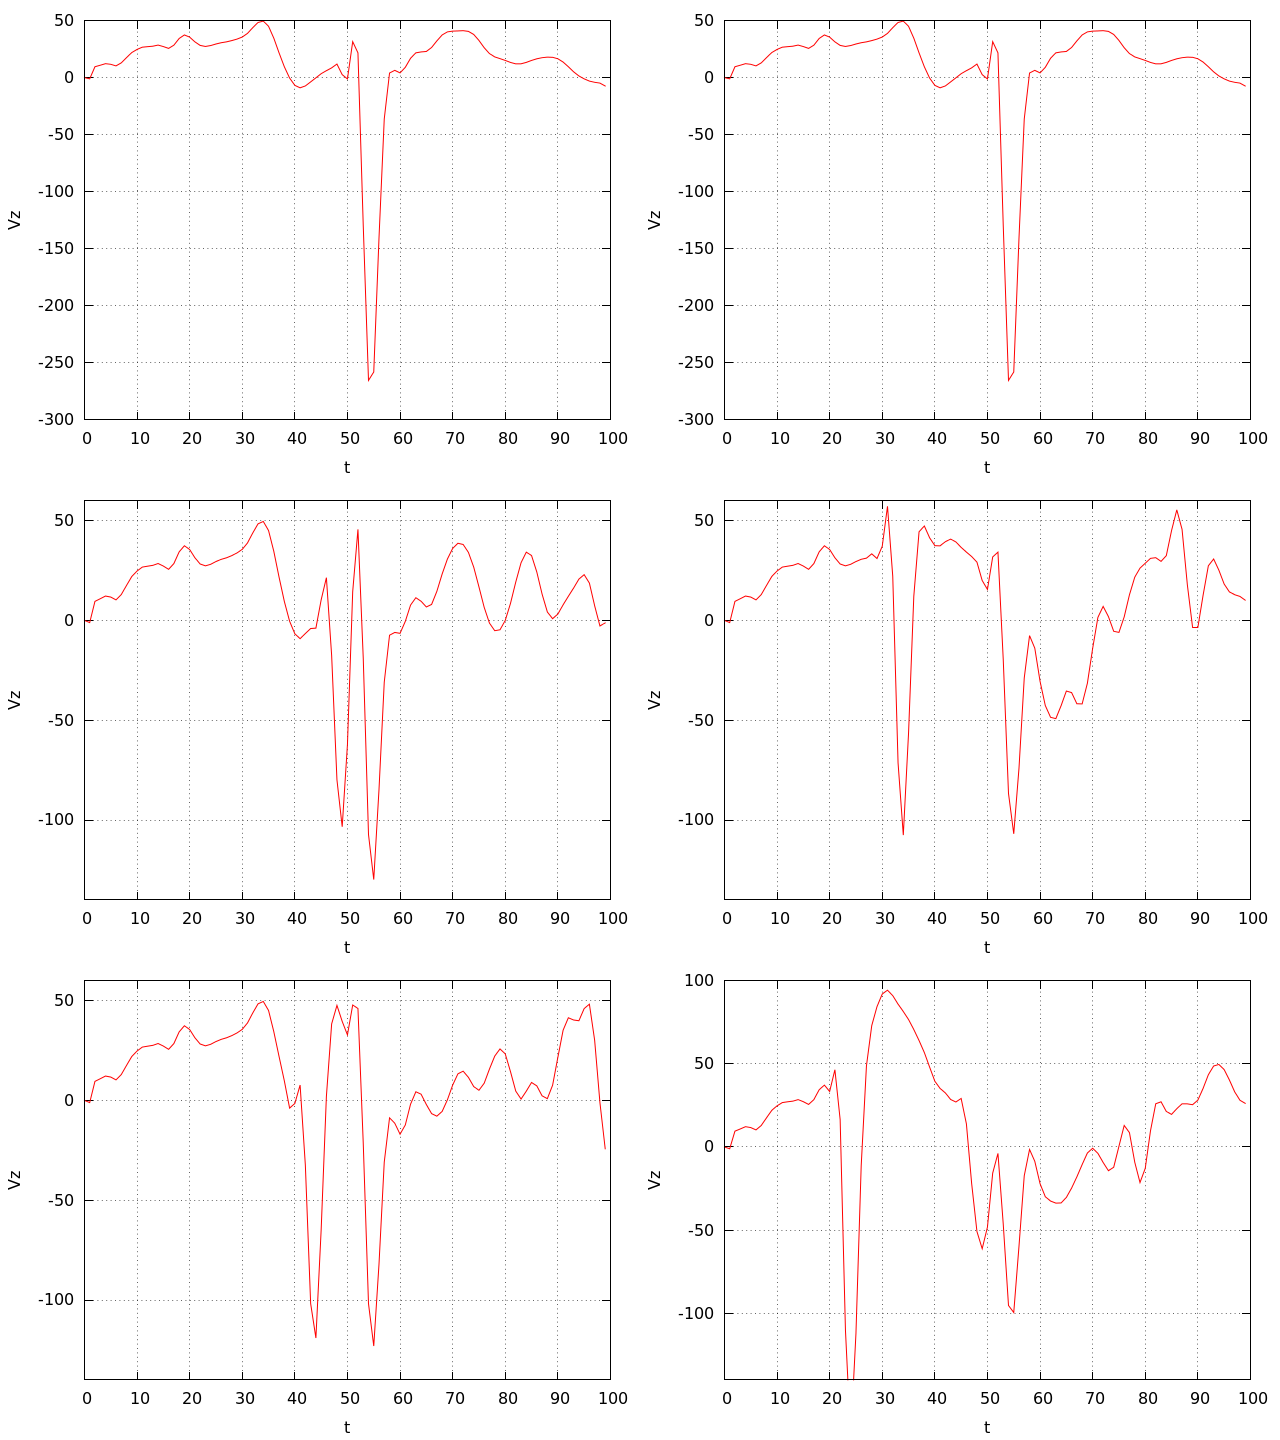
\includegraphics[width=1\textwidth]{png/res/fracture-detection.png}}
	\caption{Показания ультразвукового датчика на продольных возмущениях. Слева сверху вниз -- отклик для материала без расслоения, для материала с расслоением между 1-м и 2-м снизу слоями, для материала с расслоением между 2-м и 3-м снизу слоями. Справа сверху вниз -- отклик для материала без расслоения, для материала с расслоением между 4-м и 5-м снизу слоями, для материала с расслоением между 6-м и 7-м снизу слоями. Всего слоёв 11}
	\label{pic:fracture-detection}
\end{figure}

На рис. \ref{pic:s-wave-detector} показаны рассчитанные показания ультразвукового детектора на сдвиговых волнах для образца без расслоения.
\begin{figure}%[H]
	\center{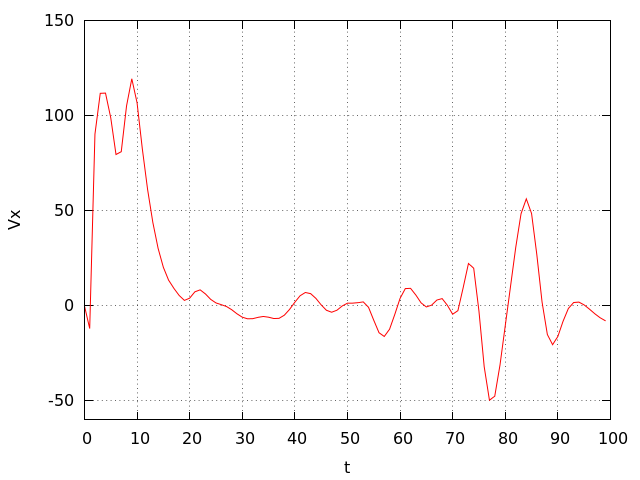
\includegraphics[width=0.7\textwidth]{png/res/s-wave-detector.png}}
	\caption{Показания ультразвукового датчика на сдвиговых возмущениях. Отклик для материала без расслоения. Сильное зашумление и затухание сигнала}
	\label{pic:s-wave-detector}
\end{figure}

Предыдущие расчёты сделаны для образца из 11-ти слоёв. Можно провести расчёт и для 22-x слоёв (рис. \ref{pic:22layers}). Границы между слоями можно видеть по скачкам значений давления, обусловленным разными скоростями распространения волн в плоскости изображённого среза. Метод и в этом случае позволяет детектировать отслоение тыльного слоя -- рис. \ref{pic:22-detector}.

\begin{figure}%[H]
	\center{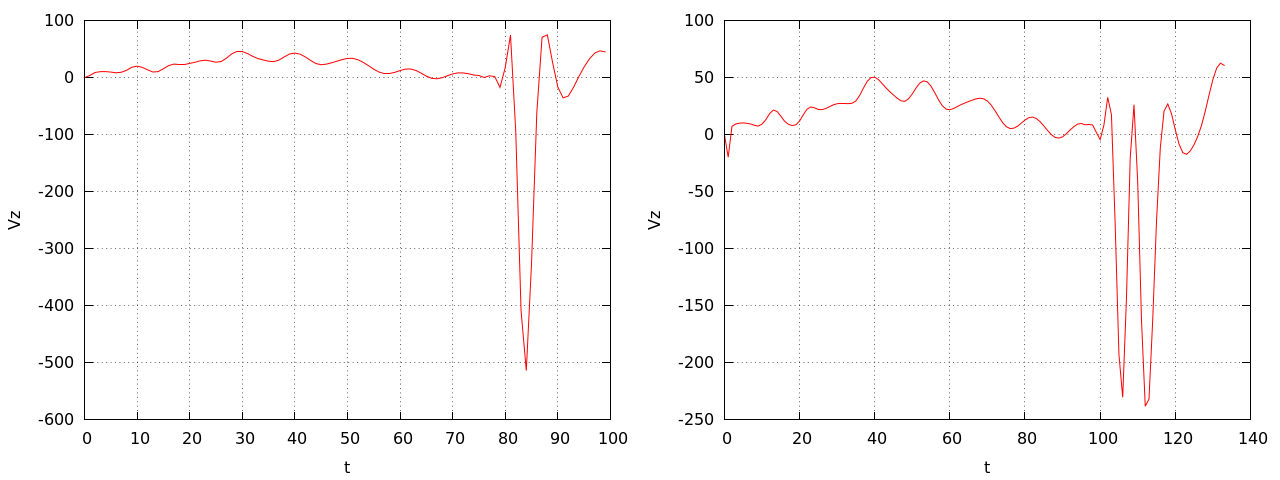
\includegraphics[width=1\textwidth]{png/res/22-detector.png}}
	\caption{Показания ультразвукового датчика на продольных возмущениях для материала с 22-мя слоями. Слева материал без трещины, справа -- материал с расслоением между 1-м и 2-м снизу слоями. Метод позволяет разрешить отслоение тыльного слоя}
	\label{pic:22-detector}
\end{figure}

\begin{figure}%[H]
	\center{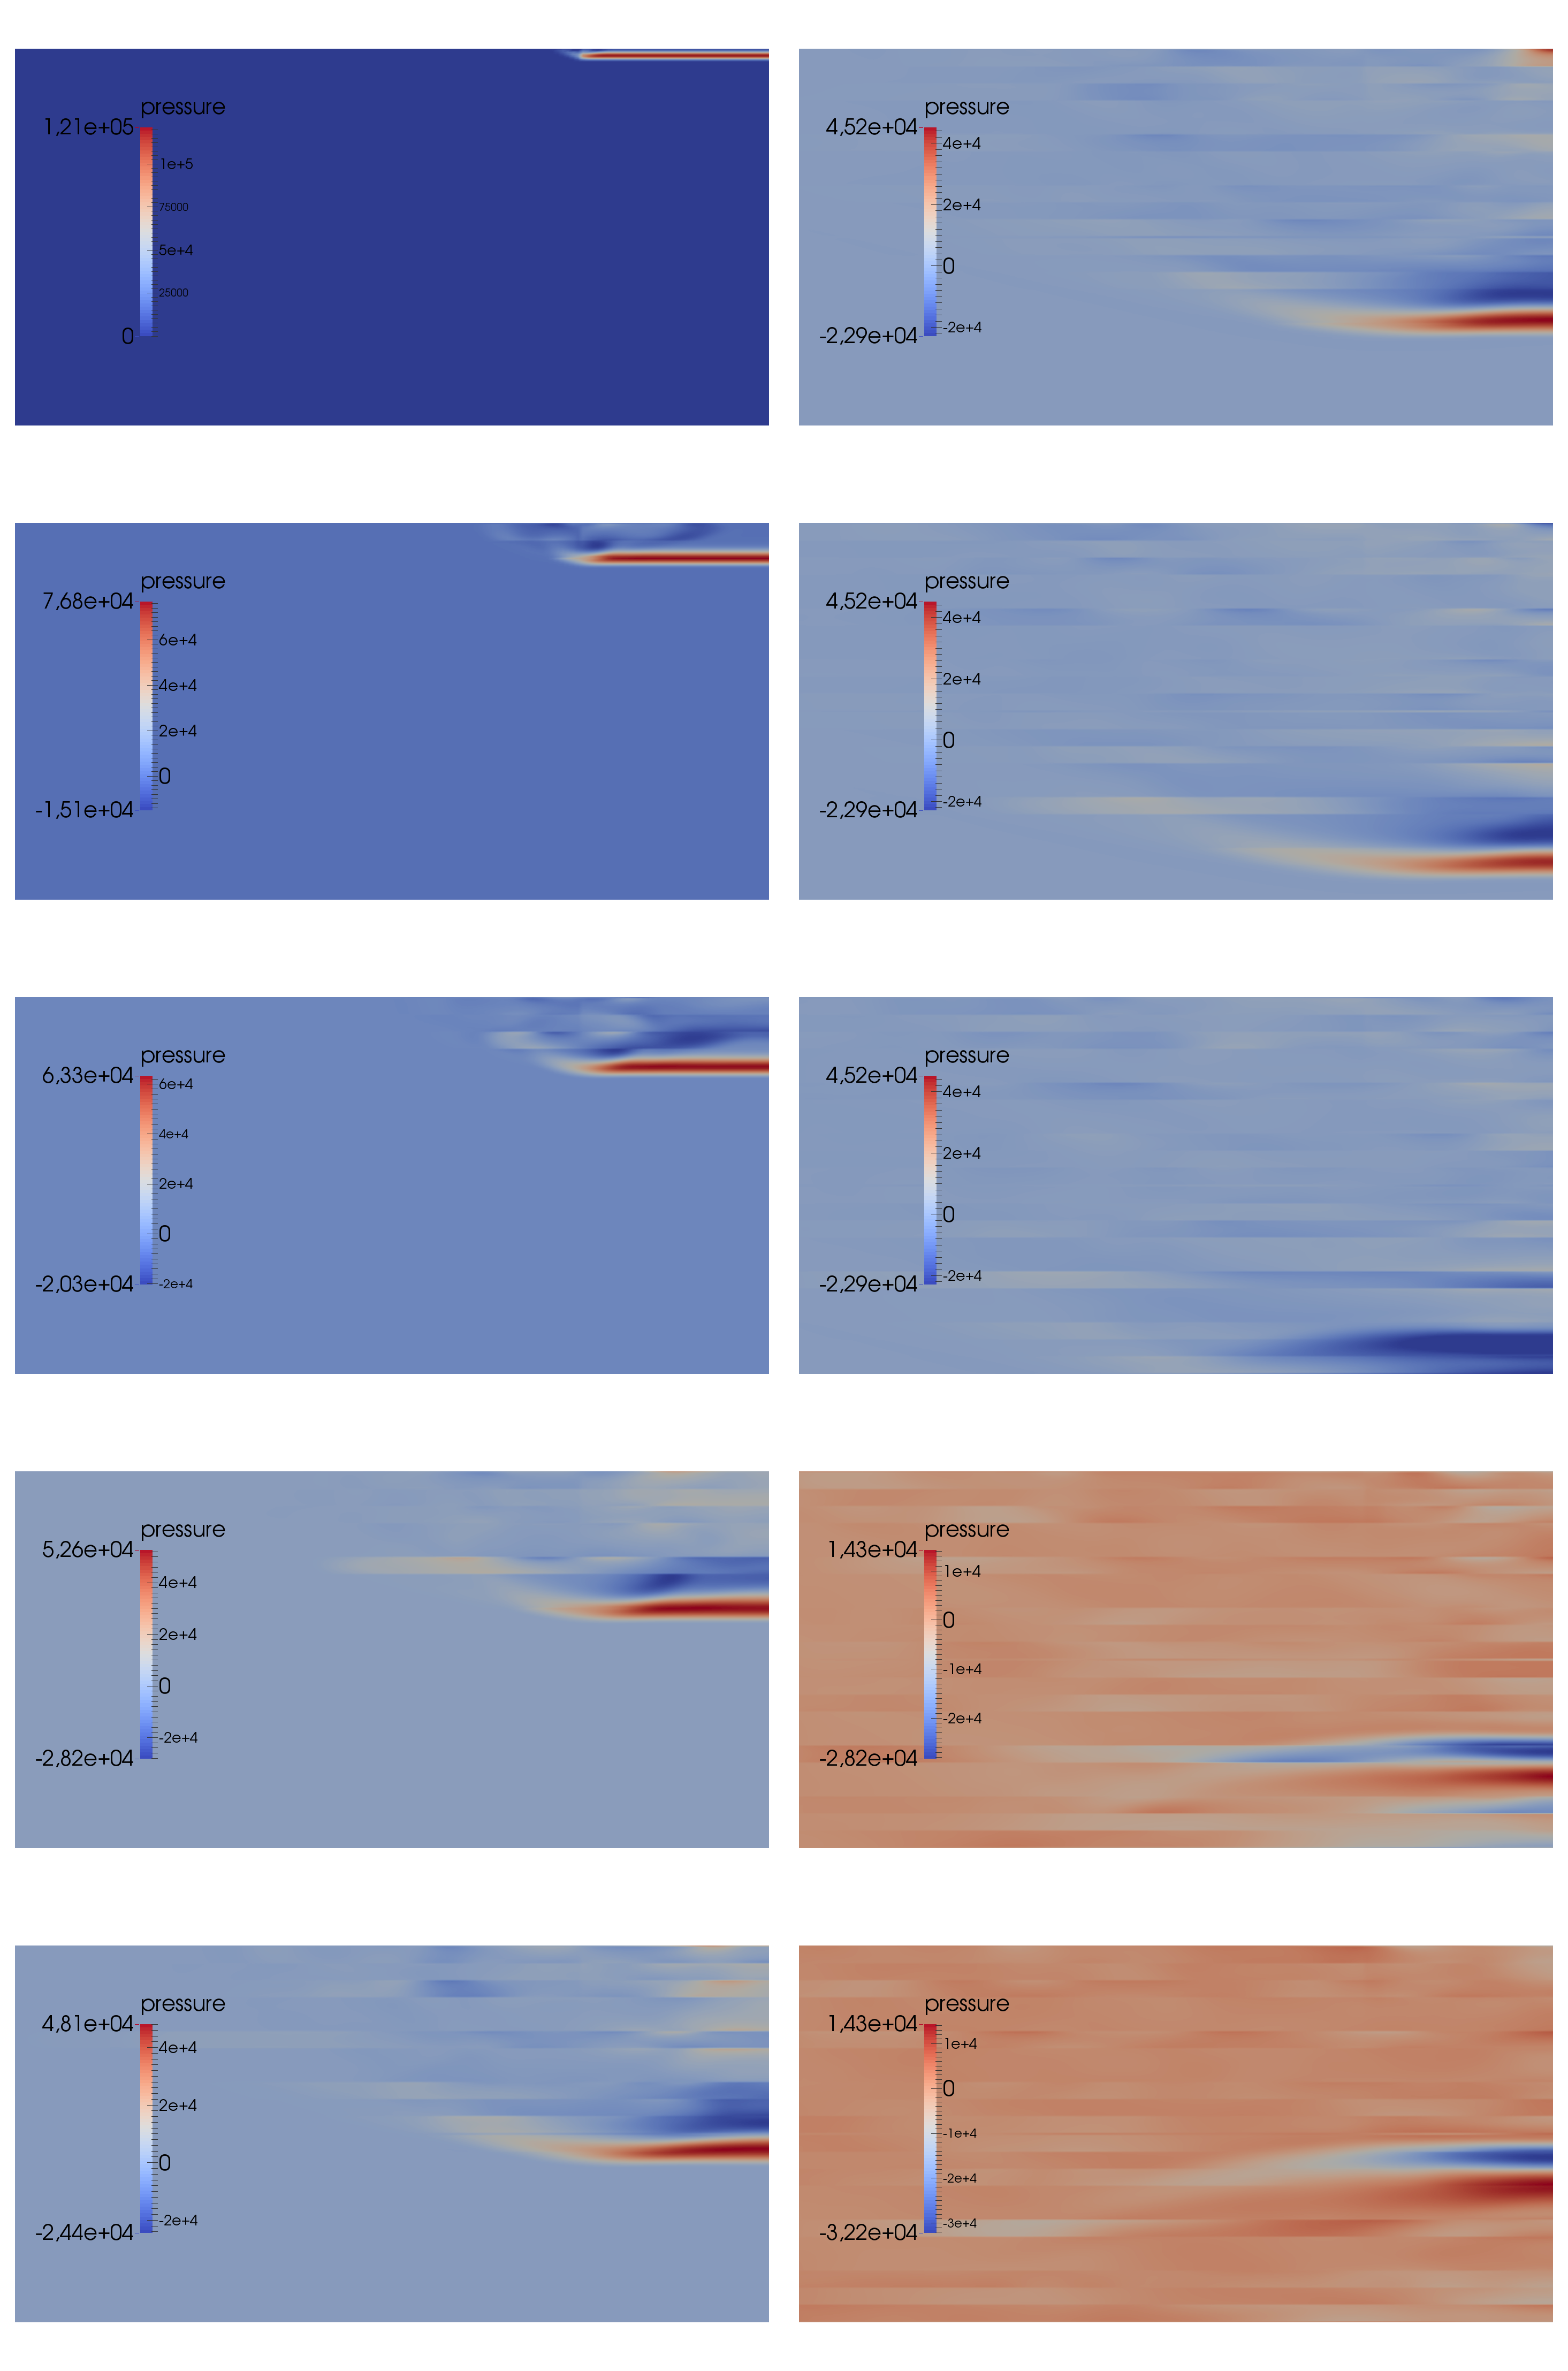
\includegraphics[width=1\textwidth]{png/res/22layers.png}}
	\caption{Половина поперечного среза образца с 22-мя анизотропными слоями. Последовательные моменты времени сверху вниз, слева направо}
	\label{pic:22layers}
\end{figure}

\subsection{Верификация результатов}
Для представленных выше расчётов была проконтролирована сходимость решения при измельчении расчётной сетки и уменьшении шага по времени. На рис. \ref{pic:convergence-szz} показан профиль отражённой от тыльной поверхности образца продольной волны для разной грубости расчётной сетки. Для той же последовательности уменьшения расчётных шагов на рис. \ref{pic:convergence-detector} представлены показания ультразвукового детектора.

\begin{figure}%[H]
	\center{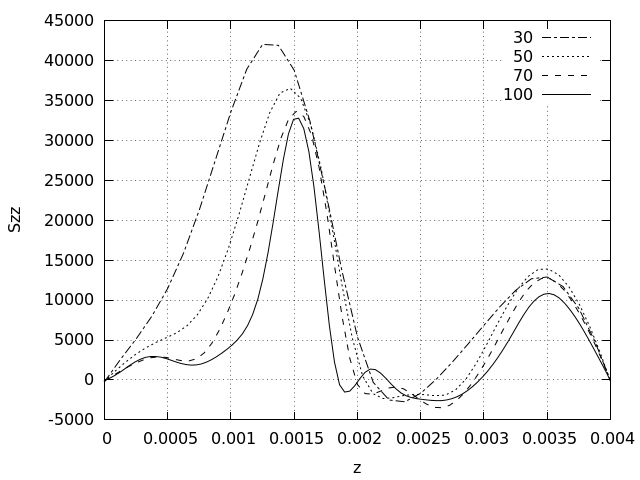
\includegraphics[width=0.9\textwidth]{png/res/convergence-szz.png}}
	\caption{\small{Сходимость в пространстве. Разными линиями показаны результаты для сеток различной мелкости (на графиках указано количество точек вдоль оси $z$)}}
	\label{pic:convergence-szz}
\end{figure}

\begin{figure}%[H]
	\center{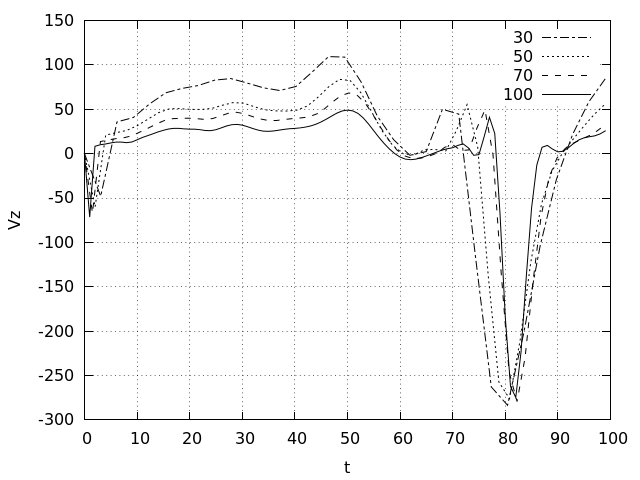
\includegraphics[width=0.9\textwidth]{png/res/convergence-detector.png}}
	\caption{\small{Сходимость во времени. Разными линиями показаны результаты для сеток различной мелкости (на графиках указано количество точек вдоль оси $z$)}}
	\label{pic:convergence-detector}
\end{figure}

Для прохождения волны через границу раздела двух сред с различными упругими свойствами было проведно сравнение численных расчётов с аналитическими формулами, выписанными в \ref{analytical_amplitudes}. Получено совпадение результатов в широких пределах варьирования отношения упругих модулей и плотностей.


\subsection{Расчёты на неструктурированной расчётной сетке}
\subsubsection{Расчёты на треугольной расчётной сетке}
Были проведены расчёты постановок неразрушающего контроля в двумерном приближении на треугольной сетке -- промоделировано отражение волны от внутреннего дефекта произвольной формы -- рис. \ref{pic:2d}.
\begin{figure}%[H]
	\center{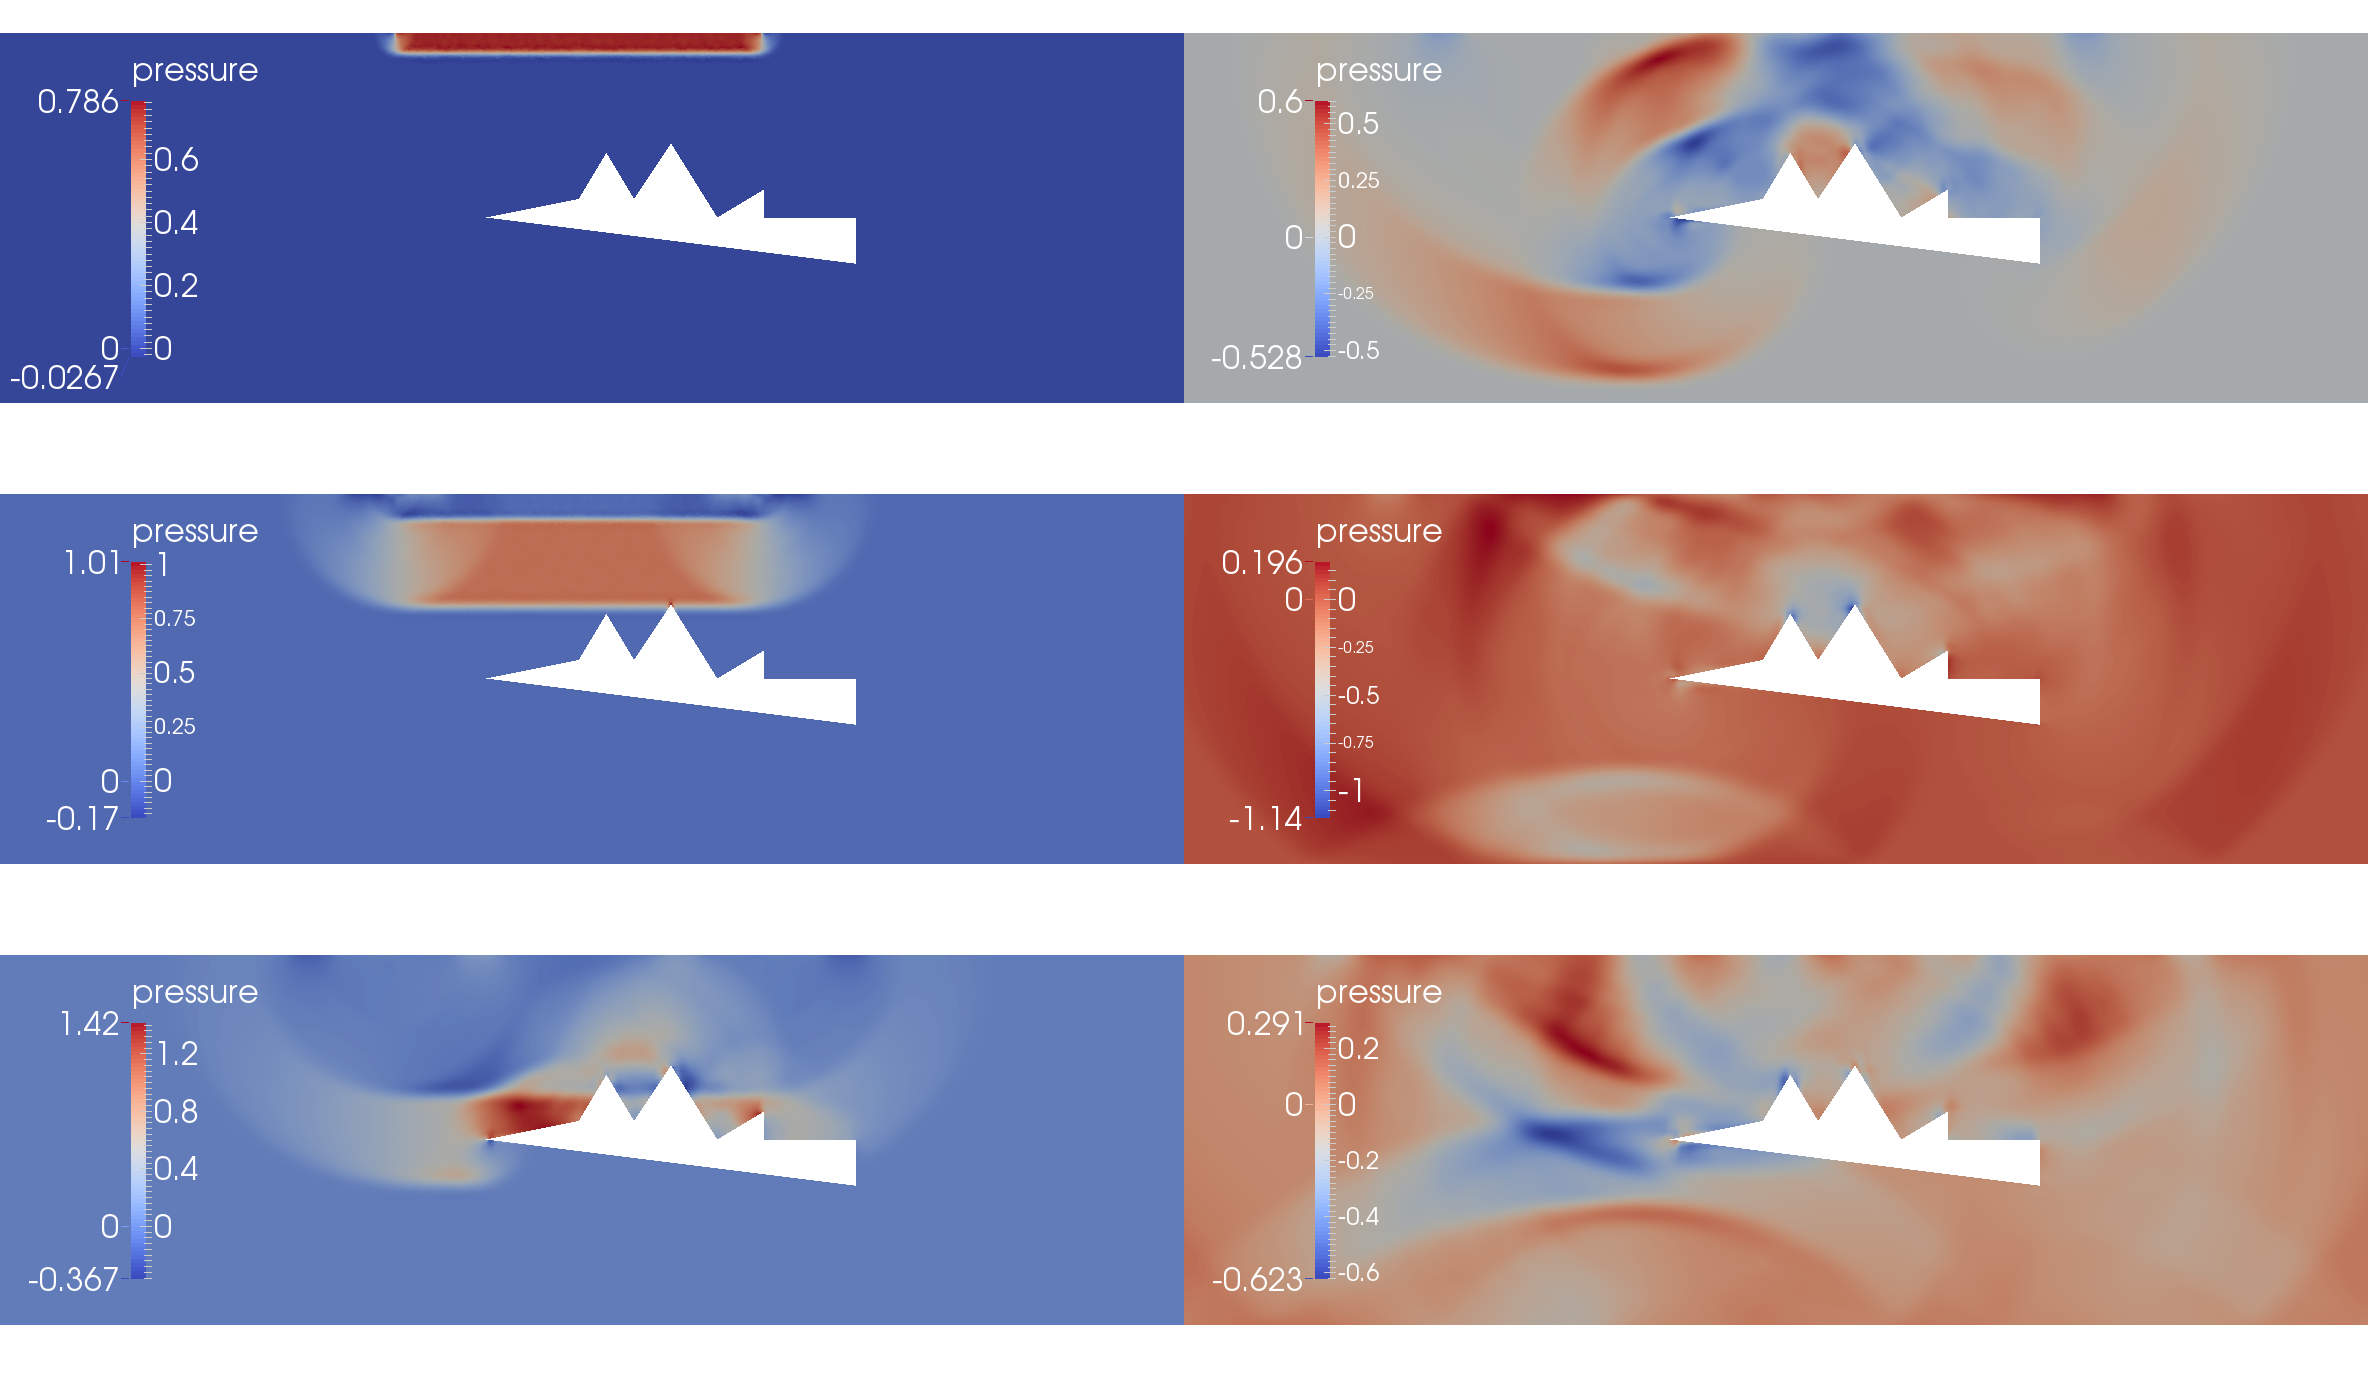
\includegraphics[width=1\textwidth]{png/res/2d.png}}
	\caption{Расчёт неразрушающего контроля образца с дефектом произвольной формы на треугольной сетке. Последовательные моменты времени сверху вниз, слева направо}
	\label{pic:2d}
\end{figure}

\subsubsection{Расчёты на тетраэдрической расчётной сетке}
В данный момент идёт работа для возможности проведения серийных расчётов на трёхмерной неструктурированной сетке. Пока представим лишь результаты отдельных расчётов. На рис. \ref{pic:layers-tetr} показан расчёт неразрушающего контроля образца с внутренним дефектом произвольной формы. На рис. \ref{pic:icosahedron-3d-view} и \ref{pic:icosahedron-2d-view} показан расчёт модельной постановки -- взрыв внутри изотропного икосаэдра. Взрыв задаётся начальным условием фиксированного давления.
\begin{figure}%[H]
	\center{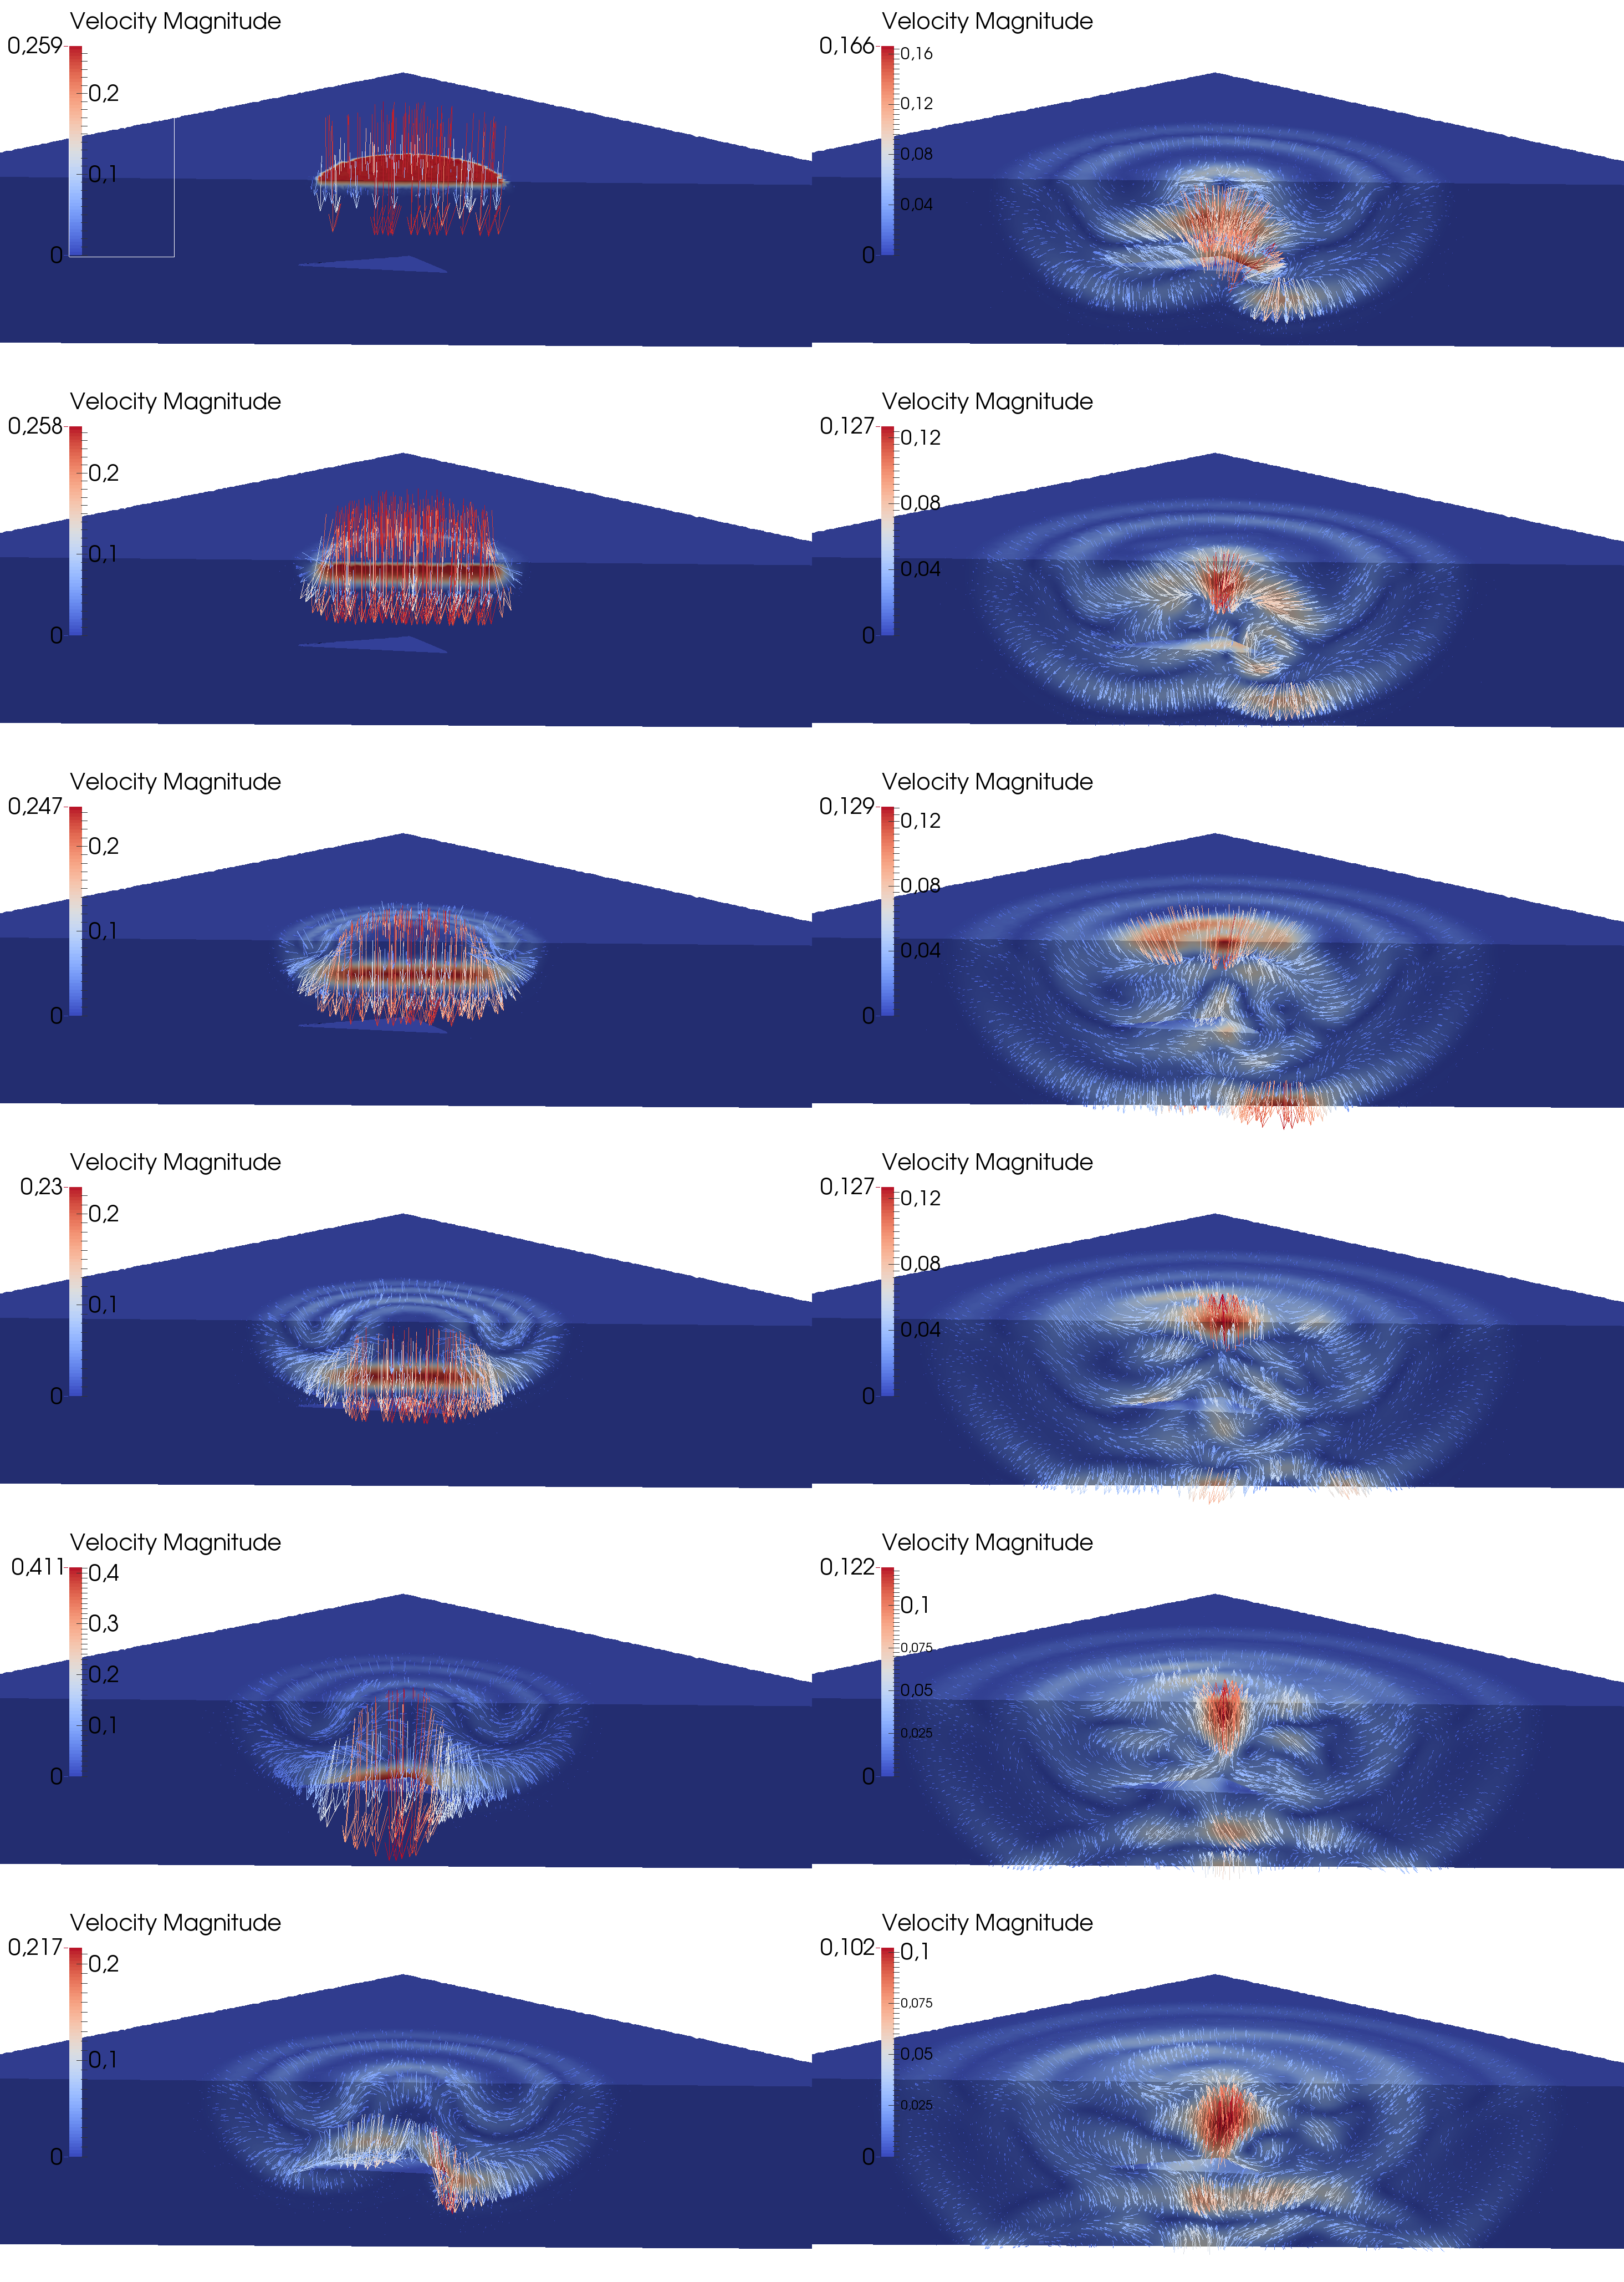
\includegraphics[width=1\textwidth]{png/res/layers-tetr.png}}
	\caption{Расчёт неразрушающего контроля образца с дефектом произвольной формы на тетраэдрической сетке. Последовательные моменты времени сверху вниз, слева направо}
	\label{pic:layers-tetr}
\end{figure}

\begin{figure}%[H]
	\center{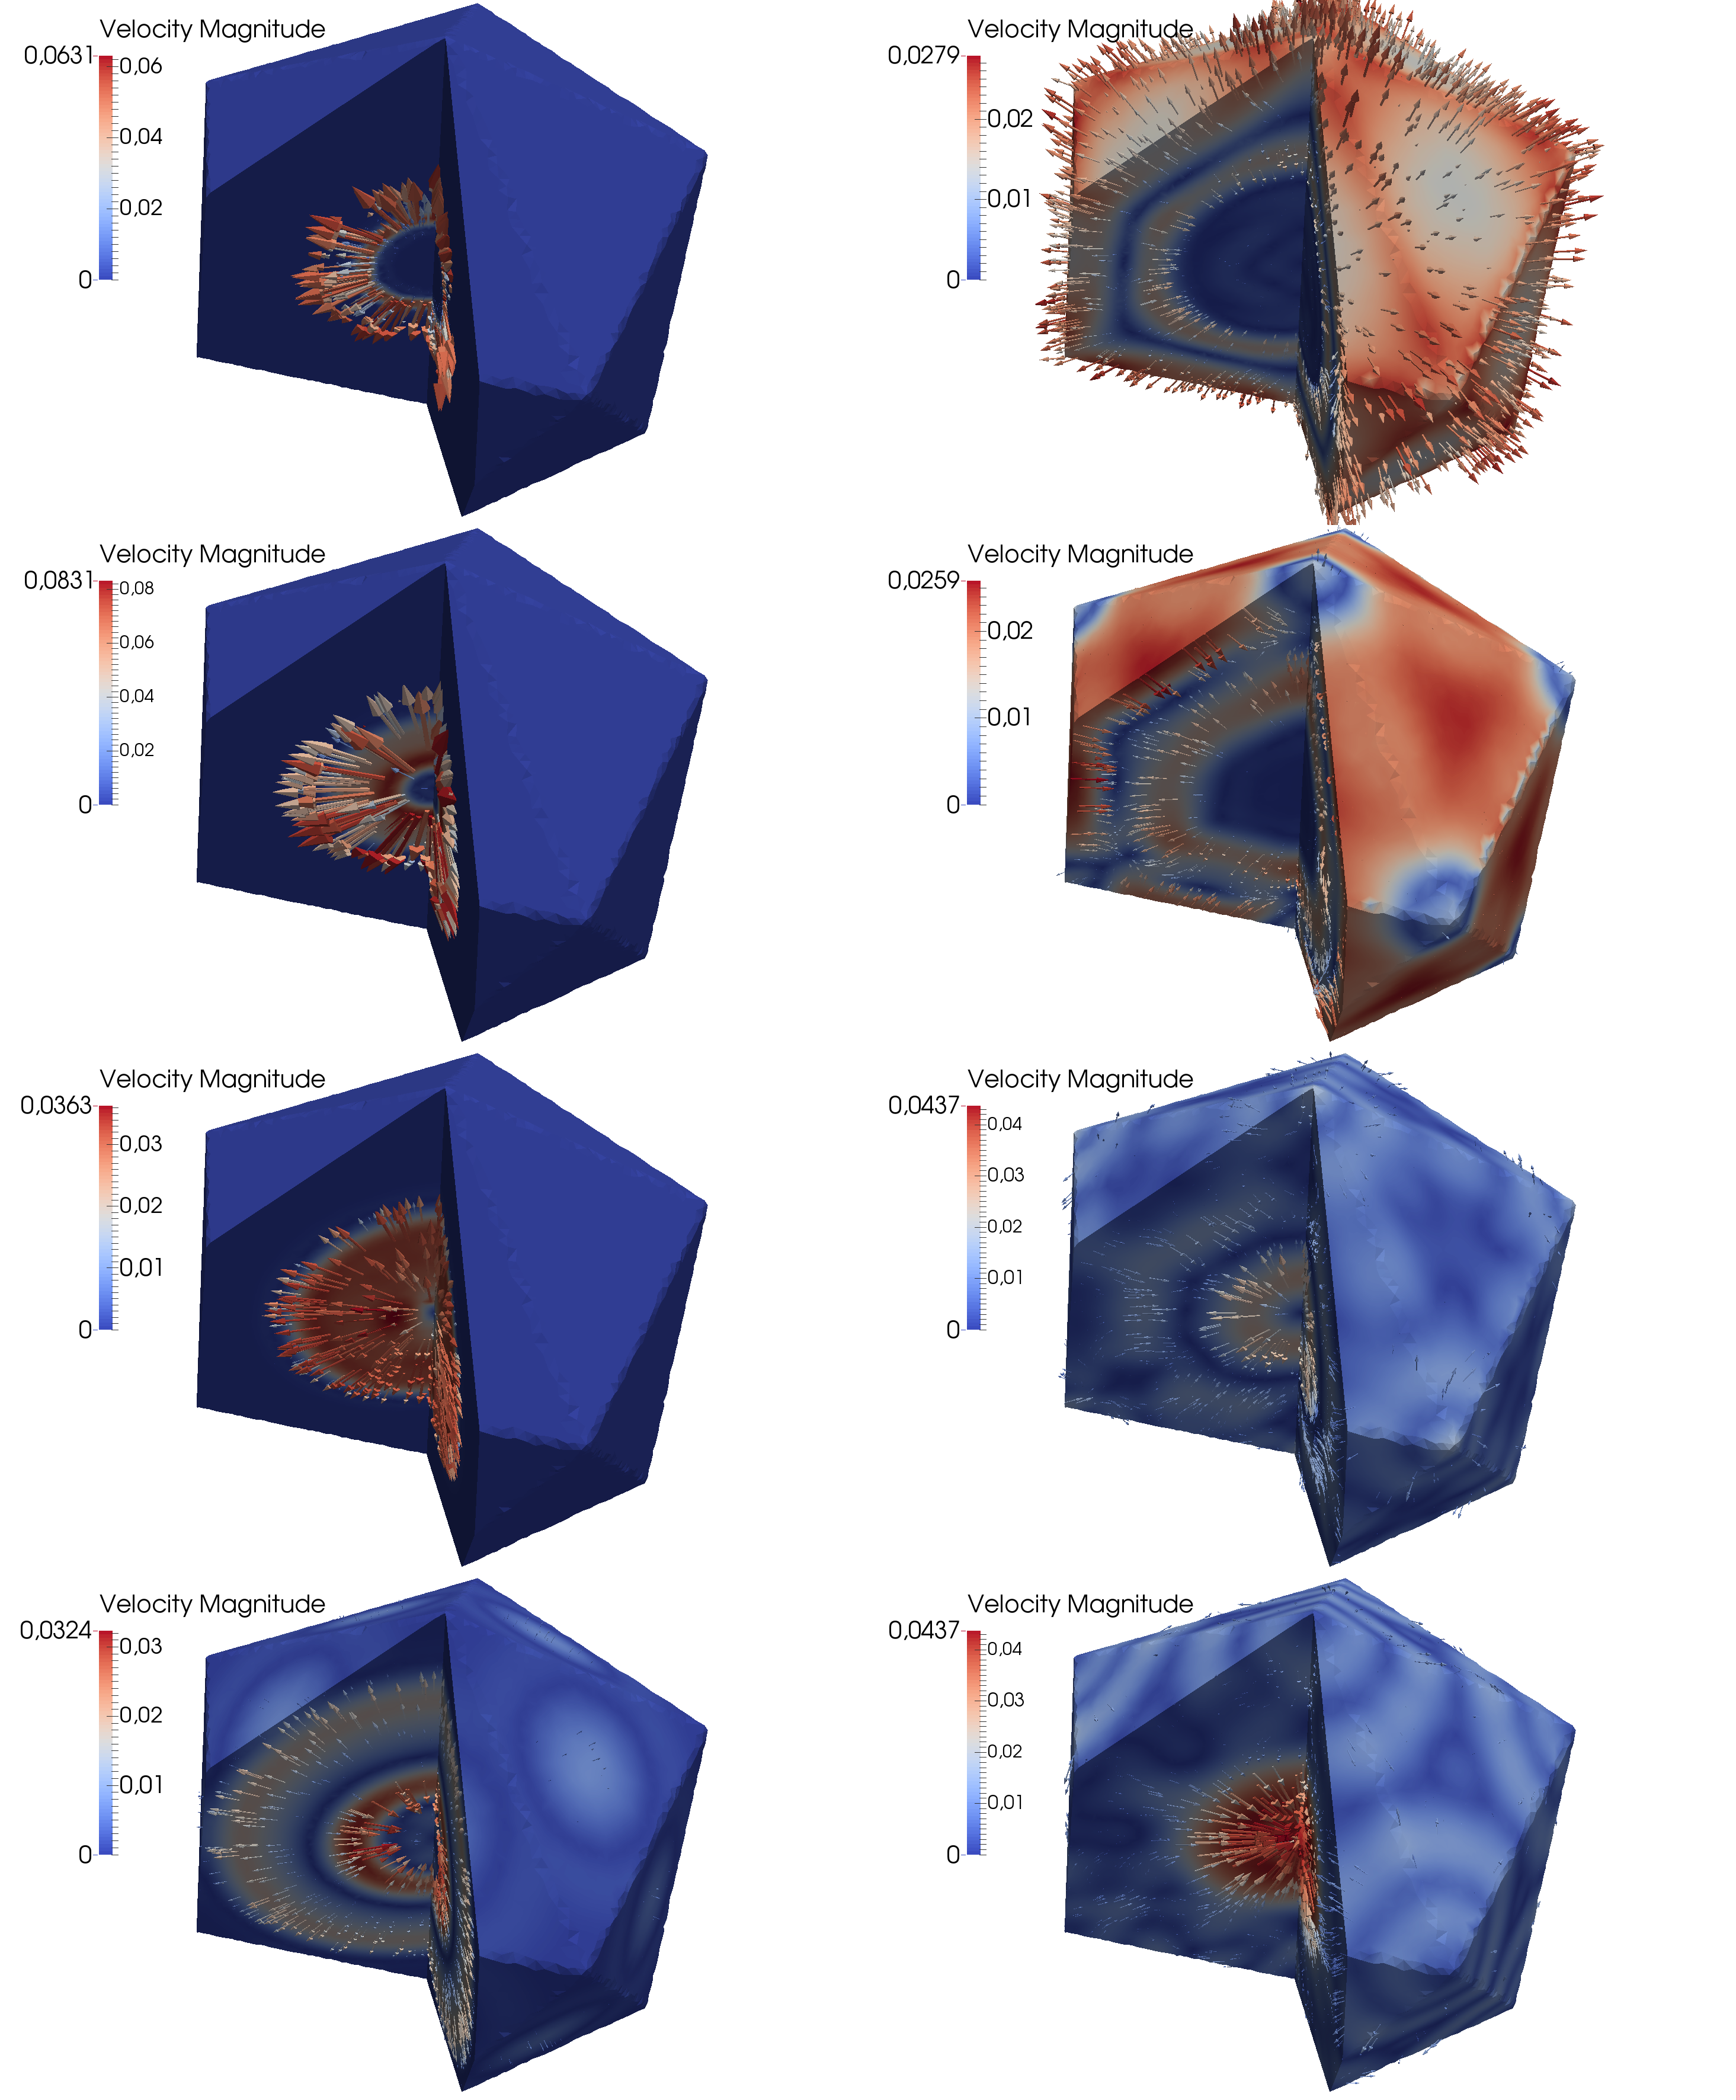
\includegraphics[width=1\textwidth]{png/res/icosahedron-3d-view.png}}
	\caption{Расчёт взрыва в икосаэдре на неструктурированной сетке. Последовательные моменты времени сверху вниз, слева направо}
	\label{pic:icosahedron-3d-view}
\end{figure}

\begin{figure}%[H]
	\center{\includegraphics[width=1\textwidth]{png/res/icosahedron-2d-view.png}}
	\caption{Расчёт взрыва в икосаэдре на неструктурированной сетке - двумерный срез. Последовательные моменты времени сверху вниз, слева направо}
	\label{pic:icosahedron-2d-view}
\end{figure}














